\chapter{Asking Billionaires How They Got RICH!}

We begin here with a different sort of mathematical object. There is no blackboard, no formal derivation in the usual sense, and no validated frame on which we can rest a visible equation. Instead, the lecture builds its arithmetic in the street: a G-Wagon, a Ferrari, a football owner, a doctor, a restaurant operator, and a sequence of short encounters from which a business logic slowly emerges. What matters is not the luxury object itself, but the operating structure beneath it: persistence, delegation, ROI, retained earnings, working capital, leverage, and the difference between money that exists on paper and money that is actually available.

Unless otherwise stated, bare dollar quantities that appear in equations below are measured in millions of dollars.

\section{River Oaks, Wealth Signals, and the Search Problem}

The lecture opens with a teaser montage of wealth signals. We hear fragments: a G-Wagon owner connected to football, a doctor with a large annual number, and the promise that somebody might tell us how one comes to own a Ferrari in 2024. These fragments are not yet the content. They are bait, and they are meant to be. The lecture is staging a question before it answers it.

Only after this quick prologue does the field itself come into view. Houston is described as one of the world's great concentrations of millionaires, and River Oaks is named as the immediate terrain. Within the logic of the lecture, this functions as a sampling premise:
\begin{equation}
\operatorname{rank}_{\text{millionaire-city}}(\text{Houston}) = 8.
\end{equation}
We should read that less as a theorem than as the stated reason for the experiment. The host is not wandering randomly. He is choosing a neighborhood in which the visible markers of wealth are likely to correlate with large-scale business experience.

The important conceptual move comes right here. A luxury car is treated as a pointer, not as an explanation. We first find the external sign, and only then do we ask what business machinery, what discipline, and what risk lay underneath it.

\section{The Search Rule: Refusal Before Advice}

The lecture then does something useful: it keeps the refusals. A number of early approaches fail. People decline, brush the host off, or give him only a second before moving on. Those moments are not waste. They establish the first operating principle of the chapter. Before there is any business theorem, there is a search theorem: access is scarce, so persistence is part of the method.

The host turns the setback into a rule. Every no is framed as movement toward a yes. That principle is not abstract optimism. It is the lecture's first piece of process discipline. One continues the search, not because success is guaranteed, but because the search cannot function if refusal is treated as a final judgment.

The first small payoff comes through the restaurant-owner exchange, and its content is deliberately compressed. We are given several short maxims:
\begin{itemize}
\item be fearless,
\item do not be afraid to fail,
\item if a business is to scale at all, a good product must still be present underneath the rest of the story.
\end{itemize}
We also hear a quantitative anchor: the restaurant owner names a largest annual business figure of about \(12\) in our units, that is, about twelve million dollars a year. The exchange remains terse, almost resistant, but that terseness matters. The lecture is teaching us how to listen. When later interviews elaborate cash management or financing, they will not be replacing this early advice. They will be supplying the mechanism that these compressed aphorisms lack.

\section{The Texans Interview: Scale, Entry, and Cash Conservatism}

The lecture now returns to one of its opening hooks and lets it unfold properly. The owner of the Houston Texans becomes the first major case, and the tone changes immediately. We are no longer hearing a quick street remark about grit. We are hearing a higher-level owner asked to account for entry into an extremely competitive field, for advice received from mentors, and for the role of money in seizing opportunity.

The first answer is still a slogan: never quit. But the lecture does not allow the slogan to float by itself. It asks what previous business success made this possible, what industry came first, and what maxim governed the use of money. The answer is short and blunt: conserve your cash. The interview therefore begins to connect entrepreneurial persistence to financial position.

\subsection{Question \& Answer}

\paragraph{Question.} What does persistence look like once the stakes become large?

\paragraph{Answer.} In this interview persistence is not simply psychological toughness. It is supported by prior success, by cash discipline, by a willingness to use leverage, and by the refusal to negotiate from weakness. The speaker's negotiation advice can be expressed in the minimal form
\begin{equation}
V_{\text{deal}} \geq V_{\text{walk}},
\end{equation}
where \(V_{\text{walk}}\) denotes the value of the live outside option. If walking away has no value because one is desperate, then the bargaining position is hollow.

\begin{remark}
The phrase ``conserve your cash'' has the same structure. Opportunities do not arrive on a schedule. Cash is what allows an owner to act when a discontinuous opening appears.
\end{remark}

The transcript then performs an important didactic turn. The host pauses and restates the lesson in his own words: people often quit when they are very near the thing they want. That recap must remain in the chapter. Without it, the Texans segment becomes a set of isolated answers. With it, the lecture extracts a principle and prepares us for the next case, where the arithmetic becomes denser.

\section{The Ferrari Interview I: From Self-Employment to Organization}

After the recap, the lecture returns to the street and begins its most substantial interview. We are now with an entrepreneur in labor-force management, and the questioning narrows quickly toward scale. How important was delegation? How important was team-building? What is the difference between a founder doing everything and a business that grows beyond the founder?

\begin{definition}
In the language of this lecture, a founder is \emph{self-employed} when output remains bottlenecked by the founder's own labor. A business becomes \emph{scalable} when organization allows the enterprise to live and grow beyond any one person.
\end{definition}

The interview then gives the sharpest quantitative contrast in the lecture. In annual terms,
\begin{align}
R_{\text{company}} &\approx 300,\\
R_{\text{solo}} &\approx 3,\\
\frac{R_{\text{company}}}{R_{\text{solo}}} &\approx 100.
\end{align}
The last line is editorial compression, not a law of management. It serves one purpose only: to make the order-of-magnitude jump unmistakable. The point is that organization changes the ceiling by roughly two orders of magnitude.

\subsection{Question \& Answer}

\paragraph{Question.} What separates self-employment from a business that can actually scale?

\paragraph{Answer.} The lecture's answer is organizational before it is financial. A single person can only do so much. Therefore we must identify the founder's limitations, surround them with complementary strengths, and build a team that executes on the founder's behalf. Only then does the venture become something other than a job the founder has built for himself.

This is why the interview insists on a distinction that ordinary business talk often blurs. A profitable individual operation may be admirable, but it is not yet the same thing as a company that can outlive the founder's daily labor. The lecture wants that distinction made sharply, because the financial discussion that follows depends on it.

\section{The Ferrari Interview II: ROI, Paper Wealth, and Working Capital}

Once scale is on the table, the lecture tightens. It does not jump immediately to debt. First it lays down a spending rule. Every dollar spent inside the business must have an ROI attached to it. In cleaned notation we may write
\begin{equation}
\mathrm{ROI}_i=\frac{\Delta \Pi_i}{C_i},
\end{equation}
where \(C_i\) is expenditure \(i\) and \(\Delta \Pi_i\) is the incremental gain attributed to it. The interview never writes this formula, of course, but the formula captures the spoken rule: business spending is to be treated as investment, not decoration.

From there the lecture makes a deeper move. It asks whether the entrepreneur has ever been broke, and the answer is not the usual one. The speaker says yes, emphatically so, and then explains that one can be making a large amount of money on paper while being nearly cashless in personal terms.

\subsection{Question \& Answer}

\paragraph{Question.} How can somebody make millions and still be broke in cash terms?

\paragraph{Answer.} The lecture gives a concrete example. In the units fixed above,
\begin{equation}
Y_{\text{paper}} \approx 3,\qquad T \approx 0.95,\qquad C_{\text{personal}} \approx 0.01.
\end{equation}
That is, about three million dollars recognized, about nine hundred fifty thousand dollars owed in tax, and only about ten thousand dollars sitting in the personal account.

\begin{proposition}
Large paper income need not imply large personal liquidity.
\end{proposition}

\begin{proof}
The lecture's mechanism is straightforward. Earnings are recognized and therefore taxed. At the same time, the cash itself is needed inside the company if the company is still growing and financing its own expansion. Hence the owner's economically relevant cash may remain trapped inside the business while the tax obligation has already been triggered. In symbols,
\[
Y_{\text{paper}} \neq C_{\text{personal}}.
\]
The inequality is conceptual rather than accounting-complete, but it expresses the lecture's central paradox exactly.
\end{proof}

The transcript then continues in the correct order. Having established the paradox, it asks how the business was funded in the first place. The answer is: badly, expensively, and under pressure. There was no initial pile of capital. There was invoice factoring, high-interest borrowing, and a discipline of leaving profit in the firm rather than taking it out.

Let \(E_t\) denote retained earnings, \(P_t\) periodic profit, \(D_t\) owner withdrawals, and \(B_t\) borrowed working capital. The lecture's repair mechanism can be written as
\begin{align}
E_{t+1} &= E_t + P_t - D_t,\\
B_{t+1} &= B_t - (P_t - D_t).
\end{align}
During the repair phase the speaker is describing, distributions are essentially shut down,
\begin{equation}
D_t \approx 0,
\end{equation}
so that profitable operation implies
\begin{equation}
B_{t+1} \approx B_t - P_t < B_t
\qquad \text{whenever } P_t>0.
\end{equation}
This is the lecture's central update rule in business-finance language. Each profitable period that is not drained by withdrawals reduces the need for outside capital in the next period.

Now the financing path itself becomes visible. The entrepreneur describes invoice factoring at roughly \(21\%\) and later bank credit at roughly \(6\%\) to \(8\%\):
\begin{equation}
r_{\text{factor}} \approx 0.21,\qquad r_{\text{bank}} \approx 0.06 \text{ to } 0.08.
\end{equation}
The narrative order matters. We do not start with cheap money. We start with ugly money. Then, by retained earnings and reduced dependence on outside borrowing, the firm makes itself legible to a bank.

\begin{figure}
\centering
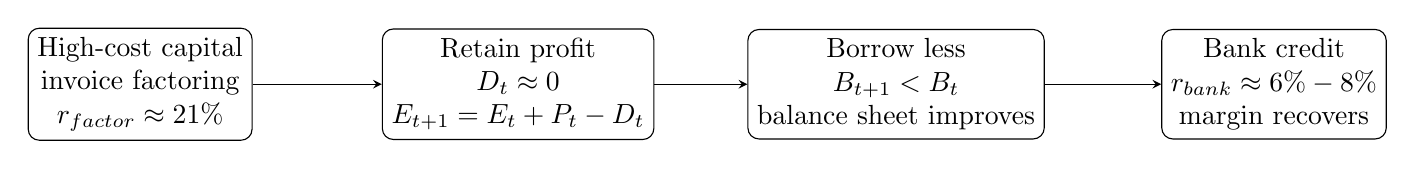
\begin{tikzpicture}[>=stealth]
\node[draw, rounded corners, align=center] (a) at (0,0) {High-cost capital\\invoice factoring\\\(r_{\text{factor}}\approx 21\%\)};
\node[draw, rounded corners, align=center] (b) at (4.8,0) {Retain profit\\\(D_t\approx 0\)\\\(E_{t+1}=E_t+P_t-D_t\)};
\node[draw, rounded corners, align=center] (c) at (9.6,0) {Borrow less\\\(B_{t+1}<B_t\)\\balance sheet improves};
\node[draw, rounded corners, align=center] (d) at (14.4,0) {Bank credit\\\(r_{\text{bank}}\approx 6\%-8\%\)\\margin recovers};
\draw[->] (a.east) -- (b.west);
\draw[->] (b.east) -- (c.west);
\draw[->] (c.east) -- (d.west);
\end{tikzpicture}
\caption{Working-capital sequence reconstructed from the Ferrari interview.}
\end{figure}

The interview also makes a quantitative claim about the payoff from refinancing the cost of capital: roughly twenty to twenty-five thousand dollars a month back to the bottom line. This invites one cautious worked example.

Let \(K\) be the financed working-capital base, measured in millions of dollars, and let \(\Delta \Pi_{\text{month}}\) be the monthly improvement in millions. Then
\begin{align}
\Delta \Pi_{\text{month}} &\approx \frac{(r_{\text{factor}}-r_{\text{bank}})K}{12},\\
K &\approx \frac{12\,\Delta \Pi_{\text{month}}}{r_{\text{factor}}-r_{\text{bank}}}.
\end{align}
If we take the midpoint values
\[
\Delta \Pi_{\text{month}} \approx 0.0225,\qquad
r_{\text{factor}}-r_{\text{bank}} \approx 0.14,
\]
then
\begin{equation}
K \approx \frac{12 \times 0.0225}{0.14} \approx 1.93.
\end{equation}
So the interview is plausibly describing a working-capital burden in the low seven figures.

\begin{remark}
This final estimate is editorial arithmetic rather than a spoken formula. It is useful because it keeps us from hearing ``twenty-five thousand a month'' as a free-floating number. The lecture is describing a real reduction in financing drag produced by internal discipline and balance-sheet repair.
\end{remark}

We may now summarize the financial chain in the order the lecture itself discovers it:
\begin{enumerate}
\item expensive short-term capital keeps the business alive,
\item retained profit reduces next period's borrowing need,
\item the balance sheet strengthens,
\item cheaper bank capital becomes available,
\item lower interest expense lifts the monthly bottom line.
\end{enumerate}
This is the most mathematically substantial part of the chapter, and the notes should linger here rather than rush past it.

\section{Final Doctrine, Interlude, and the Business of Medicine}

Before the lecture leaves the Ferrari interview, it performs one more contraction. The host asks how somebody can own a Ferrari in 2024, and the answer is reduced to two rules: find something one is genuinely passionate about, and do not quit. The lecture has earned the right to say this by now. Earlier, the same slogan might have floated. Here it sits on top of a machinery of delegation, retained earnings, and expensive financing survived.

There is then a commercial pause in the narration. The host inserts a short announcement about the School of Mentors and then resets the inquiry. This interlude is not part of the analytic spine, but it is part of the lecture's rhythm: a pause, a reset, and then one final street approach.

The final interview is with a doctor who also owns a substantial business. This matters because the lecture now broadens its claim. We are no longer speaking only of founders in the obvious entrepreneurial sense. We are speaking of a professional whose craft sits inside a business system.

The doctor distinguishes personal medical income from the size of the broader business:
\begin{equation}
A_{\text{medicine}} \approx 0.6 \text{ to } 0.7,\qquad
A_{\text{practice}} \approx 6,\qquad
N_{\text{employees}} \approx 300.
\end{equation}
The precise accounting category of each number is not fully specified in the transcript, so it is better to preserve the lecture's distinction than to force stricter bookkeeping labels onto it.

\subsection{Question \& Answer}

\paragraph{Question.} Why must even medicine be understood as a business system?

\paragraph{Answer.} The lecture's answer is not that medicine should be reduced to money. It is that efficient care, payroll, practice survival, and long-run service are coupled. If the practice fails as an organization, then the physician cannot sustainably perform the professional work at all.

The doctor's warning is therefore subtle and important. Young doctors often fail to learn the business of medicine, not because they are greedy, but because they imagine they can remain purely clinical while someone else silently solves the organizational problem. The lecture refuses that separation. Private practice means payroll, niche, efficiency, and solvency. If those collapse, patient care suffers with them.

\begin{remark}
This closing case is what prevents the chapter from becoming a simple mythology of flashy entrepreneurship. The same business disciplines reappear inside a respectable profession: cash flow, operational efficiency, and the need to stay afloat.
\end{remark}

The lecture ends, then, not by glorifying luxury, but by widening the domain of business literacy. One may be a founder, a franchise owner, a restaurateur, or a physician; the underlying requirement is similar. If the institution is to endure, somebody must understand its economics.

\section{Summary}

The lecture begins with surface signals and ends with hidden structure. It first teaches us how to search: keep moving through refusals until a serious conversation appears. It then teaches us how to listen: do not stop at slogans such as ``never quit'' or ``be fearless,'' but ask what financial and organizational conditions make those slogans survivable.

The Texans interview ties persistence to cash conservatism, leverage, and the ability to walk away from a bad bargain. The Ferrari interview carries the main mathematical payload: one person versus an organization, ROI attached to spend, income on paper versus personal liquidity, retained earnings as an update rule, and the transition from \(21\%\) invoice-factoring money to \(6\%\) to \(8\%\) bank money. The doctor interview then generalizes the lesson: even a high-status profession becomes a business system once payroll, efficiency, and survival come into view.

The strongest compression of the chapter is therefore this: wealth is the visible shell, but the lecture keeps leading us back to a handful of operating laws. Build organization. Conserve cash. Attach return to spending. Retain profit while the firm is fragile. Lower the cost of capital when the balance sheet permits it. Learn the business mechanics of the field one inhabits. Only then do the visible symbols begin to make any sense at all.